\documentclass[11pt]{article}

\usepackage{exscale}
\usepackage{graphicx}
\usepackage{amsmath}
\usepackage{latexsym}
\usepackage{times,mathptm}
\usepackage{epsfig}
\usepackage{tikz}

\textwidth 6.5truein          
\textheight 9.0truein
\oddsidemargin 0.0in
\topmargin -0.6in


\parindent 0pt          
\parskip 5pt
\def\baselinestretch{1.1}

\begin{document}

\begin{LARGE}
\centerline {\bf CSci 423 Homework 10}
\end{LARGE}
\vskip 0.25cm

\centerline{\bf\Large Due: 12:30 pm, Thursday, 12/5}
\centerline{Daniel Quiroga}

Collaborators: Ethan Young, Will Elliot, Yang Zhang, Kevin Li

\begin{enumerate}

\item (5 points) Prove that PCP is solvable (or decidable) over the alphabet $\Sigma=\{1\}$ by giving a pseudocode algorithm. \newline
I will use dominoes to solve the PCP problem\newline
Algorithm:
We look through the dominoes:
\begin{enumerate}
\item If there some dominoe that has the same number of 1's on the top and bottom we will accept. 
\item If we find a dominoe with more 1's on top than on the bottom (say a difference of x) and then vice versa (more on the bottom than top) with a difference of y. By taking y dominoes of the first and x dominoes of the second we have the same number of 1's on both the top and bottom. meaning we have a match and accept. 
\item the last case is when all of the dominoes have more on top than on the bottom (or vice versa) then we reject. 
\end{enumerate}
since there is an algorithm that solves this we can say PCP is solvable.

\item (10 total points, 1 point for each answer) Closure properties of {\bf P} and {\bf NP}.

\begin{enumerate}
\item Is {\bf P} closed under union, intersection, concatenation, complement and star?
Just answer "yes" or "no" for each operation.\newline 
union: yes\newline 
intersection: yes\newline
concatenation: yes\newline
complement: yes\newline
star: yes\newline
\item Is {\bf NP} closed under union, intersection, concatenation, complement and star?
Just answer "yes" or "no" for each operation.\newline 
union: yes\newline 
intersection: yes\newline
concatenation: yes\newline
complement: no\newline
star: yes\newline
\end{enumerate}


\item (5 points) This problem considers an attempt at a polynomial reduction from one problem to another that does not work. Your task is to find the flaw. 
A bipartite graph is an undirected graph in which every cycle has even length. We attempt to show that the Hamiltonian cycle (a cycle that passes through each node exactly once) problem polynomially reduces to the Hamiltonian cycle problem in bipartite graphs. We need a function $T$: 
\{graphs\}$\rightarrow$\{bipartite graphs\} such that T can be computed in polynomial time and for any graph $G$, $G$ has Hamiltonian cycle iff $T(G)$ has a Hamiltonian cycle. Let $T(G)$ be the bipartite graph obtained by inserting a new vertex on every edge. Use a graph $G$ with {\bf four} nodes to show what is wrong with this transformation.\newline 
\begin{right}
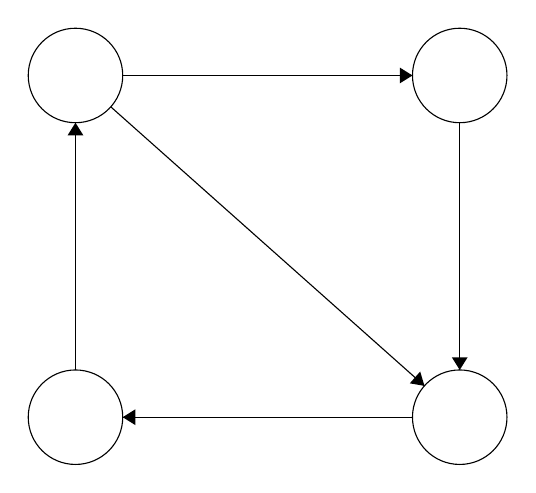
\begin{tikzpicture}[scale=0.2]
\tikzstyle{every node}+=[inner sep=0pt]
\draw [black] (26.7,-17.1) circle (3);
\draw [black] (26.7,-38.8) circle (3);
\draw [black] (51.1,-17.1) circle (3);
\draw [black] (51.1,-38.8) circle (3);
\draw [black] (29.7,-17.1) -- (48.1,-17.1);
\fill [black] (48.1,-17.1) -- (47.3,-16.6) -- (47.3,-17.6);
\draw [black] (51.1,-20.1) -- (51.1,-35.8);
\fill [black] (51.1,-35.8) -- (51.6,-35) -- (50.6,-35);
\draw [black] (48.1,-38.8) -- (29.7,-38.8);
\fill [black] (29.7,-38.8) -- (30.5,-39.3) -- (30.5,-38.3);
\draw [black] (26.7,-35.8) -- (26.7,-20.1);
\fill [black] (26.7,-20.1) -- (26.2,-20.9) -- (27.2,-20.9);
\draw [black] (28.94,-19.09) -- (48.86,-36.81);
\fill [black] (48.86,-36.81) -- (48.59,-35.9) -- (47.93,-36.65);
\end{tikzpicture}
\end{right}

\newline
$\downarrow \downarrow \downarrow \downarrow \downarrow \downarrow \downarrow \downarrow \downarrow \downarrow \downarrow \downarrow \downarrow \downarrow \downarrow \downarrow \downarrow \downarrow \downarrow \downarrow \downarrow \downarrow \downarrow \downarrow \downarrow \downarrow \downarrow \downarrow \downarrow \downarrow \downarrow \downarrow \downarrow \downarrow \downarrow \downarrow$
\newline \newline 
\begin{right}
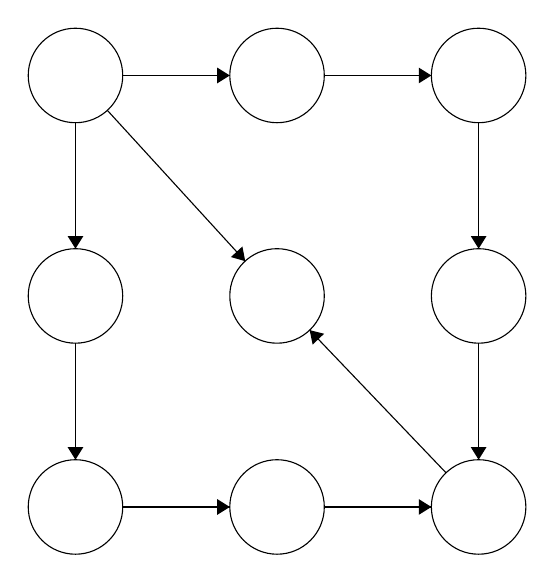
\begin{tikzpicture}[scale=0.2]
\tikzstyle{every node}+=[inner sep=0pt]
\draw [black] (38,-12.3) circle (3);
\draw [black] (25.2,-39.7) circle (3);
\draw [black] (25.2,-12.3) circle (3);
\draw [black] (25.2,-26.3) circle (3);
\draw [black] (50.8,-26.3) circle (3);
\draw [black] (50.8,-39.7) circle (3);
\draw [black] (38,-26.3) circle (3);
\draw [black] (38,-39.7) circle (3);
\draw [black] (50.8,-12.3) circle (3);
\draw [black] (25.2,-15.3) -- (25.2,-23.3);
\fill [black] (25.2,-23.3) -- (25.7,-22.5) -- (24.7,-22.5);
\draw [black] (50.8,-29.3) -- (50.8,-36.7);
\fill [black] (50.8,-36.7) -- (51.3,-35.9) -- (50.3,-35.9);
\draw [black] (25.2,-29.3) -- (25.2,-36.7);
\fill [black] (25.2,-36.7) -- (25.7,-35.9) -- (24.7,-35.9);
\draw [black] (28.2,-39.7) -- (35,-39.7);
\fill [black] (35,-39.7) -- (34.2,-39.2) -- (34.2,-40.2);
\draw [black] (41,-39.7) -- (47.8,-39.7);
\fill [black] (47.8,-39.7) -- (47,-39.2) -- (47,-40.2);
\draw [black] (28.2,-12.3) -- (35,-12.3);
\fill [black] (35,-12.3) -- (34.2,-11.8) -- (34.2,-12.8);
\draw [black] (41,-12.3) -- (47.8,-12.3);
\fill [black] (47.8,-12.3) -- (47,-11.8) -- (47,-12.8);
\draw [black] (50.8,-15.3) -- (50.8,-23.3);
\fill [black] (50.8,-23.3) -- (51.3,-22.5) -- (50.3,-22.5);
\draw [black] (27.22,-14.51) -- (35.98,-24.09);
\fill [black] (35.98,-24.09) -- (35.8,-23.16) -- (35.07,-23.83);
\draw [black] (48.73,-37.53) -- (40.07,-28.47);
\fill [black] (40.07,-28.47) -- (40.26,-29.39) -- (40.99,-28.7);
\end{tikzpicture}
\end{right} \newline 
Using the algorithm described, I noticed that the Hamiltonian graph does not exist in the second graph since depending on which path you take you will miss at least one node in the graph and thus does not fulfill the characteristics of a Hamiltonian graph.



\item(4, 6 points) Consider the following two similar graph coloring problems.

{\bf 3-Color}\\
INSTANCE: Graph $G=(V, E)$.\\
QUESTION: Can the nodes in $G$ be colored with up to 3 colors such that no two nodes connected by an edge are given the same color?

{\bf 4-Color}\\
INSTANCE: Graph $G=(V, E)$.\\
QUESTION: Can the nodes in $G$ be colored with up to 4 colors such that no two nodes connected by an edge are give the same color?

It is known that {\bf 3-Color} is NP-complete. Prove that {\bf 4-Color} is NP-complete in the following two steps.

\begin{enumerate}

\item Prove {\bf 4-Color} is in {\bf NP}. \newline 
Algorithm: \newline
For each node check each connecting edge. If any edge contains a node with the same color reject. Else continue on through the graph until you have visitied each node. \newline 
As you are visiting each node, make sure that there are 4 or less colors, if for any reason there is a fifth color we reject the graph since it is not 4-Color.  \newline 
Since there is a polynomial time solution we can say that 4-color is in NP.
\item Prove that {\bf 3-Color} reduces to {\bf 4-Color}.\newline
Say we have a graph that satifies 3-color, we call it C. C' will be created from the original C, where C' is 4-color. For each node in C we will add an edge that gives a node with a new color n. Since all the nodes will only add a node colored n, we know that it will satisfy 4-color and can simply be reversed to 3-color by taking out all nodes colored n. Since they can be worked back and forth we know that 3-color reduces to 4-color. 

\end{enumerate}


\item (5 bonus points) The problem {\bf X} is defined as follows:

PROBLEM {\bf X}\\
INSTANCE: Finite sets $A_1,\ldots,A_m$ and $B_1,\ldots,B_n$.\\
QUESTION: Is there a set $T$ such that $|T\cap A_i|\ge 1$ for $i=1,\ldots,m$ and $|T\cap B_j|\le 1$ for $j=1,\ldots,n$

Show how SAT reduces to {\bf X} by filling out the following blanks.

In SAT, let $x_1,\ldots,x_n$ be the boolean variables. Let $c_1,\ldots,c_m$ be the clauses. Let $\phi=\land_{i=1}^m c_i$
\begin{enumerate}
\item $B_j=\{\qquad\qquad\}$ for $j=1,\ldots,n$
\item $A_i=\{\qquad\qquad\}$ for $i=1,\ldots,m$
\end{enumerate}


\end{enumerate}

\end{document}